% Compile with XeLaTeX!

\documentclass{wc-article}

% Common packages
\usepackage[UTF8]{ctex}
\usepackage[utf8]{inputenc} % allow utf-8 input
\usepackage[T1]{fontenc}    % use 8-bit T1 fonts
\usepackage{microtype}
\usepackage{times}
\usepackage{graphicx}
\usepackage{acronym}
\usepackage{tikz}
\usetikzlibrary{shapes,arrows}
\usepackage{enumitem}
\usepackage[pagebackref=true,breaklinks=true,colorlinks]{hyperref}
\usepackage{xspace}
\usepackage{setspace}
\usepackage[skip=3pt,font=small]{subcaption}
\usepackage[skip=3pt,font=small]{caption}
\usepackage{amsmath}
\usepackage[capitalise]{cleveref}
\usepackage{booktabs,tabularx,colortbl,multirow,array,makecell}
% \usepackage{overpic,wrapfig}
\usepackage{xparse}
\usepackage{indentfirst}
\setlength{\parindent}{2em}
\usepackage{xltxtra}

\usepackage{setspace}

\linespread{1.5}
\zihao{5}

% 我们正在努力适配清华大学社科学报的文献注释规范!
% \usepackage[backend=refer,style=verbose-trad2]{biblatex}
% \addbibresource{reference.bib}
% \usepackage{gbt7714}
\usepackage{pifont}
\renewcommand\thefootnote{\ding{\numexpr171+\value{footnote}}}%roman

\makeatletter
\newcommand*{\rom}[1]{\expandafter\@slowromancap\romannumeral #1@}

% 使用 Arial、Times New Roman 字体
\setromanfont{Times New Roman}
\setsansfont{Arial}
\setmonofont{Courier New}

\usepackage{float}
\usepackage{listings}
\usepackage{xparse}

\hypersetup{pdfencoding=auto,colorlinks=true,allcolors=black}

% Handy shorthand
\makeatletter
\DeclareRobustCommand\onedot{\futurelet\@let@token\@onedot}
\def\@onedot{\ifx\@let@token.\else.\null\fi\xspace}
\def\eg{\emph{e.g}\onedot} 
\def\Eg{\emph{E.g}\onedot}
\def\ie{\emph{i.e}\onedot} 
\def\Ie{\emph{I.e}\onedot}
\def\cf{\emph{c.f}\onedot} 
\def\Cf{\emph{C.f}\onedot}
\def\etc{\emph{etc}\onedot} 
\def\vs{\emph{vs}\onedot}
\def\wrt{w.r.t\onedot} 
\def\dof{d.o.f\onedot}
\def\etal{\emph{et al}\onedot}
\makeatother

% Text Color
\newcommand*{\red}{\textcolor{red}}
\newcommand*{\green}{\textcolor{green}}
\newcommand*{\blue}{\textcolor{blue}}
\newcommand*{\gray}{\textcolor{gray}}
\definecolor{gray}{gray}{0.9}

\setlength\floatsep{0.5\baselineskip plus 3pt minus 2pt}
\setlength\textfloatsep{0.5\baselineskip plus 3pt minus 2pt}
\setlength\dbltextfloatsep{0.5\baselineskip plus 3pt minus 2pt}
\setlength\intextsep{0.5\baselineskip plus 3pt minus 2pt}

\makeatother

% Clever references
\crefname{algorithm}{算法}{算法}
\Crefname{algorithm}{算法}{算法}
\crefname{section}{小节}{小节}
\Crefname{section}{小节}{小节}
\crefname{table}{表格}{表格}
\Crefname{table}{表格}{表格}
\crefname{figure}{图}{图}
\Crefname{figure}{图}{图}

% Acronym
\acrodef{thu}[THU]{Tsinghua University}

\title{文章标题}
\author{韩梅梅}
\id{2020000000}
\email{meimei@mails.tsinghua.edu.cn}
\department{自动化系}
\instructor{李雷}
\date{\today}

\begin{document}
\onehalfspacing

\thispagestyle{empty}

% 若要指定日期(而不是使用编译日期)落款,可以通过 \coverletter[XXXX年XX月XX日]{...} 指定。
\coverletter{
    \noindent\instructor 老师:
    
    您好!我是\department 的\author(学号:\id)。
    
    \vspace{5ex}
    
    \textit{(以下内容仅作为示例,不是必选内容,请在信件正文完成后删去)}
    \begin{itemize}
        \item{\textit{文章的主题是什么?它是如何从你的写作动机演变成终稿的主题的?}}
        \item{\textit{在修改过程中,使你最有成就感的部分是哪些?}}
        \item{\textit{在你的写作过程中,使你感到最具有挑战性的部分是什么?你是如何面对和处理这些挑战的?}}
        \item{\textit{如有可能,你还希望在哪些方面改进本文?}}
        \item{\textit{这一阶段的收获、感想、建议,一学期以来的收获、感想、建议……}}
    \end{itemize}
}

\newpage

\setcounter{page}{1}

\maketitle

\abstract{
    文章摘要,不超过300字。
}

% 3-5 个关键词
\keywords{关键词 1}{关键词 2}{关键词 3}{关键词 4}{关键词 5}

\section{终稿模板}

我们提供一份写作与沟通课程文章终稿 \LaTeX 模板,\textbf{其中文支持依赖于 \CTeX,因此在编译时,请选择 \XeLaTeX。}

我们通过 \texttt{wc-article.cls} 配置基础模板,使用 \texttt{config.tex} 编写配置。你可以自行修改其内容来方便你的使用,但请务必遵守课程最新版本的格式要求与《〈清华大学学报(哲学社会科学版)〉文献注释规范》要求,你应当从课程教师处或其他权威渠道获取它们的最新版本。本模板在 GitHub 仓库 \href{https://github.com/YuyangLee/THU-Writing-LaTeX}{YuyangLee/THU-Writing-LaTeX} 维护,如有兴趣,欢迎一起维护。

\subsection{文章撰写}

文章正文及各个区域的格式已经定义好,你只需要填充内容即可。

\subsection{文献引用}

\subsubsection{引用文献}

引用文献请以“注释”方式顺序标注,具体格式参照引用格式规范。直接或间接引用都应注明出处,编号使用带圈字符。需要注意的是,目前并没有适用于清华大学社科学报文献注释规范的 BibTeX 配置,因此我们暂时无法通过 \texttt{reference.bib} 添加参考文献。烦请手动编写文献注释内容,并通过 \texttt{footnote} 来引用。

例如(这里是一个学术期刊引文的示例)、\footnote{吴艳红:《明代流刑考》,《历史研究》2000年第6期,第33-43页。}(这里是一个注释专著引文的示例)。\footnote{戴裔煊:《〈明史·佛郎机传〉笺正》,北京:中国社会科学出版社,1984年,第6页。}

\subsubsection{参考文献}

\red{在《学报》的引用规范、脚注体例中,原则上\textbf{不会}出现文末参考文献。有特定引出点的参考文献,请在正文内使用脚注方式引用。}在正文中没有特定引出点、但对文章有参考价值的论文和专著,可汇编为“参考文献”列于文末。同样地,目前你需要手动编写参考文献条目。

文献格式按照本课程规定调整:

(1)各条文献首先按文种集中,先中文文献,后外文文献。

(2)其次按著者姓氏字顺排列。中文著作署名按照作者姓氏汉语拼音母音序排列,外文文献中译本的署名也按照作者姓名的汉语拼音母音序排列,但是按照习惯,外人姓名名在前,姓在后(尽管习惯上正文中仍然只标识姓氏);外文文献按照作者姓氏的字母顺序排列(姓氏置前,用“,”与名字隔开;多位作者只须将首位作者的姓氏前置)。 

(3)同一著者再按出版年先后排列。

\subsection{标题级次}

通过 \texttt{section}、\texttt{subsection} 和 \texttt{subsubsection} 可以使用不同级别的标题。尽量不要使用四级标题,若必须使用,请自行配置相关指令。四级标题的缩进、字体设置同第三级标题的格式,使用“(1)”“(2)”“(3)”“(4)”排序。

\subsection{图片}

图片中文字一般不大于图题,你可以通过设置 \texttt{width} 来调整图片的尺寸。示例图片见 \cref{fig:example-fig}。

\begin{figure}[H]
    \centering
    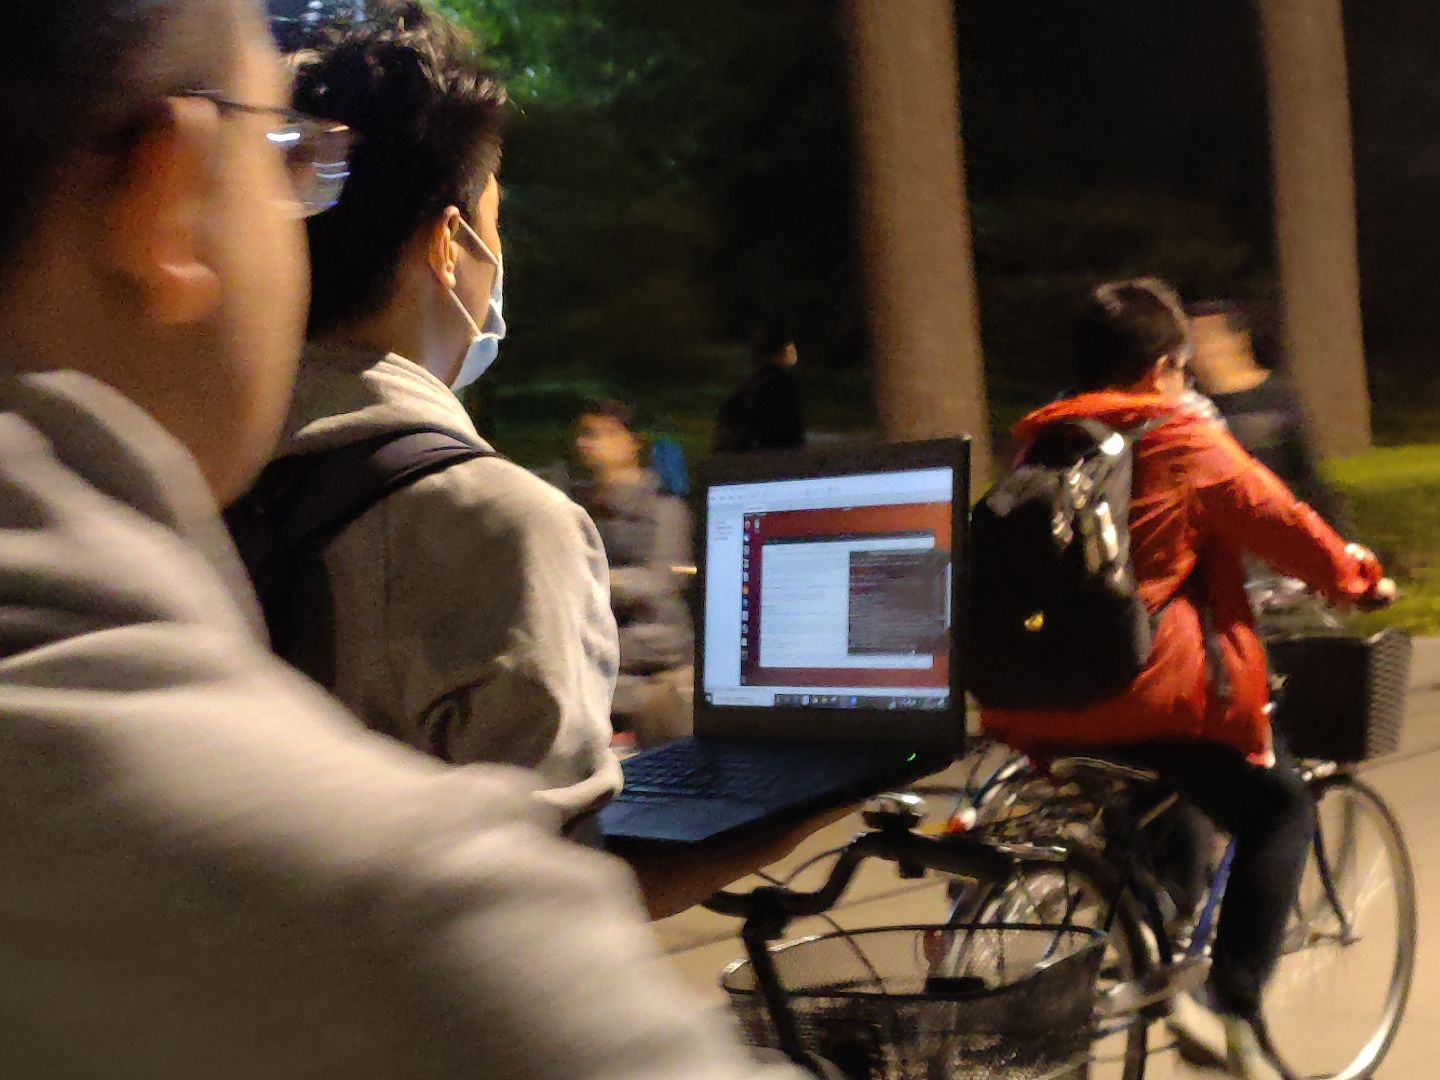
\includegraphics[width=0.5\textwidth]{assets/rider.jpg}
    \caption{一男子在学堂路上一边骑车一边使用电脑开展计算任务。}
    \label{fig:example-fig}
\end{figure}

\subsection{表格}

表格只画上框线、下框线和表头下分割线,通过 \texttt{toprule}、\texttt{midrule}、\texttt{bottomrule} 指令及 \texttt{tabular} 环境的列参数实现。示例表格见 \cref{tab:example-table}。

\begin{table}[H]
\begin{center}
    \caption{华清大学的三名同学}
    \zihao{-5}

    % 为了降低使用门槛,请手动加粗表头文本。进阶的使用者也可以通过定义 tabular format 实现。
    \begin{tabular}{c c c}
         \toprule
         \textbf{姓名} & \textbf{家乡} & \textbf{专业} \\
         \midrule
         韩梅梅 & 中国北京市海淀区 & 自动化 \\
         John Appleseed & 美国加利福尼亚州库普蒂诺 & 工业工程 \\
         Jane Smith & 英国伦敦威斯敏斯特市 & 外语言文学 \\
         \bottomrule
    \end{tabular}
\end{center}

    % 在 table 环境中编写题注,目前需要手动缩进 2 字符。
    \tabledesc{韩梅梅、John Appleseed 和 Jane Smith 是来自华清大学的三名同学。他们在 2022 年选修了清华大学《写作与沟通》课程并高度评价该课程。}
    
    \label{tab:example-table}
\end{table}


\refs{

阿尔穆特·霍弗特,2005,《中世纪晚期的国家、城市与公民》,见昆廷·斯金纳、博·斯特拉思主编:《国家与公民:历史·理论·展望》,彭利平译,上海:华东师范大学出版社。

蔡英文,2006,《公民身份的多重性——政治观念史的阐述》,见许纪霖主编:《公共性与公民观》,南京:江苏人民出版社。

马克斯·韦伯,1993,《儒教与道教》,洪天富译,南京:江苏人民出版社。

马克斯·韦伯,2004a,《韦伯作品集 \rom{2}:经济与历史·支配的类型》,康乐等译,桂林:广西师范大学出版社。

马克斯·韦伯,2004b,《韦伯作品集 \rom{3}:支配社会学》,康乐、简惠美译,桂林:广西师范大学出版社。

马克斯·韦伯,2005,《韦伯作品集:非正当性的支配——城市的类型学》,康乐、简惠美译,桂林:广西师范大学出版社。

皮埃尔·罗桑瓦龙,2005,《公民的加冕礼——法国谱选史》,吕一民译,上海:上海世纪出版集团。

唐兴霖、马骏,1999,《中国村民自治民主的制度分析》,《开放时代》第5、6月号。

Huter,J.E.,F.L.Schmidt\&G.B.Jackson,1982,Meta-analysis: Cumulating Research Findings Across Studies,Beverly Hills,CA:Sage

Isin,Engin F. \& Bryan Turner(eds.) ,2002,Handbook of citizenship Studies,London:SAGE Publications.

Marshall,T.H.,1964,Class,Citizenship and Social Development,Chicago:University of Chicago Press.

Turner,Bryan S.,2002,“Religion and Politics:The Elementary Forms of Citizenship,”in EnginIsin\& Bryan Turner(eds.),Handbook of Citizenship Studies, London:SAGE Publications.
}

\end{document}